\documentclass[runningheads]{llncs}
% Grundgröße 12pt, zweiseitig
% Standardpakete
\usepackage[utf8]{inputenc}
\usepackage[T1]{fontenc}
% deutsche Silbentrennung
\usepackage[ngerman]{babel}
\usepackage{amsmath}
\usepackage{cite}
\usepackage{float}

% Grafiken einbinden
\usepackage{graphicx}
\graphicspath{{images/}}

\usepackage{hyperref}
% tiefe des Inhaltsverzeichnisses
\setcounter{tocdepth}{2}

\title{Transaktionen}
\author{Ture Claußen, 1531067, \email{ture.claussen@stud.hs-hannover.de} \and Jannes Neemann, 1530893, \email{jannes.neemann@stud.hs-hannover.de}}
\authorrunning{T. Claußen \and J. Neemann}
\institute{Fakultät IV, Abteilung Informatik, Hochschule Hannover, Ricklinger Stadtweg 120, 30459 Hannover}


% jetzt gehts los
\begin{document}% hier gehts los{\def\addcontentsline#1#2#3{}\maketitle}
{\def\addcontentsline#1#2#3{}\maketitle} % Wird gebraucht, damit der Title nicht im Inhaltsverzeichnis steht




% \begin{center} \sffamily\bfseries Selbständigkeitserklärung \end{center}
% % fett und zentriert in der minipage

% Mit der Abgabe der Ausarbeitung erklären wir, dass wir die eingereichte Seminar-Arbeit
% selbständig und ohne fremde Hilfe verfasst, andere als die von uns angegebenen Quellen
% und Hilfsmittel nicht benutzt und die den benutzten Werken wörtlich oder
% inhaltlich entnommenen Stellen als solche kenntlich gemacht haben.
% \vspace*{7ex}

% Hannover, den \today \hfill



\begin{abstract}
  \keywords{}
\end{abstract}

\tableofcontents  % Inhaltsverzeichnis
%
%
%
\section{Einführung}
% was sind transaktionen im allgemeinen
% was sind transaktionen bei ethereum: Statemaschine
% vergelich zu bitcon
% 
Das Wort Transaktion stammt von dem lateinischen Wort \textit{transigere} ab, welches im übertragenden Sinne mit 'durchführen', 'vollführen' oder 'abmachen' (Geschäft) übersetzt werden kann. \cite{noauthor_transigere_nodate} Dieser Wortsinn besteht auch weiterhin im technischen und wirtschaftlichen Bereich, jedoch gibt es noch spezifischere Abgrenzungen. In der Wirtschaft ist es ein Vorgang bei dem Waren und Forderungen ausgetauscht werden. \cite[S. 18 f.]{ehrlicher_kompendium_1975} In der Informatik ist es im Zusammenhang mit Datenbanken eine unteilbare, \textit{atomare}, Abfolge von Anweisungen, die einen Übergang von einem konsistenten Zustand in einen Anderen beschreibt. \cite[S.520]{herold_grundlagen_2017}

Ethereum ist ein "transaktionsbasierter Automat" (\textit{transaction-based state machine}). Somit sind Transaktionen ein grundlegender Baustein von Ethereum im Allgemeinen und ihnen kommt eine ähnliche Bedeutung wie ACID Transaktionen bei. Der Automat speichert seinen Zuständ $ \sigma_t $ in der Blockchain, eine Transaktion $ T $ ist Argument der Zugstandsübergangsfunktion $ \Upsilon $, die von \textit{externen Akteuren (EA)} angestoßen wird und diesen gespeicherten Zustand $ \sigma_t $ in einen neuen, gültigen Zustand $ \sigma_{t + 1} $ überführen soll: $\sigma_{t+1} = \Upsilon(T, \sigma_t) $. Im Falle eines Konsens des Netzwerkes wird diese Zustandsveränderung durchgeführt beziehungsweise gespeichert.

Im Kontrast zu Kryptowährungen wie Bitcoin ist der Umfang des Automaten bzw. des Protokolls bei Ethereum deutlich geweitet, denn Zweck ist nicht nur die Schöpfung, Speicherung und der Austausch eines digitalen Zahlungsmittels \cite{nakamoto_bitcoin_nodate}, sondern eine allgemeine dezentrale Rechenmaschine, ein "Weltcomputer". Daher bestehen bei Ethereum auch an Transaktionen andere technische und konzeptionelle Anforderungen, die im Folgenden erläutert werden. \cite[S. 1-4]{wood_ethereum/yellowpaper_2019}

\section{Struktur und technische Umsetzung einer Transaktion}
Die Komponenten welche eine Transaktion in Ethereum ausmachen sind vergleichbar mit denen eines Briefes. Sie besitzen einen Empfänger sowie eine Frankierung, welche die Transportkosten zum Empfänger bezahlen. In einen Brief kann man z.B. Geld oder einen Text verschicken. Auch Transaktionen in Ethereum können Geld in Form von Ether und einen Text in Form von Nutzdaten verschicken. Im Weiteren wir die allgemeine Struktur und technische Umsetzung einer Transaktion vorgestellt.

\subsection{Komponenten einer Transaktion}
\label{komponenten}
Transkationen, so auch unsere Transaktion $T_x$, enthalten laut ihrer offiziellen Definition \cite[S. 4]{wood_ethereum/yellowpaper_2019} folgende Datenfelder:
\begin{description}
  \item[nonce:] Ein Skalar welcher gleich der Anzahl der vom EOA versendeten Transaktionen ist. Der Nutzen wird in \ref{nonce} erläutert.
  \item[gasPrice:] Ein Skalar der angibt, wie viel Wei man pro Einheit \textit{Gas} bezahlt, die bei der Gesamtheit aller Berechnungen die während der Ausführung der Transaktion anfallen (S. \ref{gas})
  \item[gasLimit:] Ein Skalar der die maximal Anzahl an \textit{Gas} angibt, die während der Ausführung der Transaktion verbraucht werden darf. Dieser Betrag muss im Voraus bezahlt werden.
  \item[to:] Die 160-Bit Adresse des Empfängers.
  \item[value:] Skalar der die Menge Wei angibt, die der Empfänger erhält.
  \item[v,r,s:] Komponenten der ECDSA-Signatur (S. \ref{ecdsa}), um den Sender der Transaktion zu bestimmen
  \item[init:] Ein Byte-Array unbegrenzter Länge, welches nur bei einer Kontrakterzeugung verwendet wird und den kompilierten Sourcecode des Kontrakts enthält
  \item[data:] Ein Byte-Array unbegrenzter Länge, welches die Nutzdaten des Kontrakts enthält
\end{description}


\subsection{Typen von Transaktionen}
Es gibt genau zwei Typen von Transaktion. Transaktionen die eine Nachricht von einem Account\footnote{Mit Account ist hier ein EOA oder ein Kontrakt gemeint} zu einem anderen überträgt ("`message calls"' \cite[S. 4]{wood_ethereum/yellowpaper_2019}) oder Transaktionen die einen neuen Kontrakt erzeugen ("`contract creation"' \cite[S. 4]{wood_ethereum/yellowpaper_2019})). Mit Nachricht ist dabei der Inhalt von den Feldern \textit{value} und \textit{data} gemeint.

Bei massage call Transaktionen enthält das \textit{to} Feld die öffentliche Adresse eines EOA oder eines Kontrakts. Zusätzlich besteht die Option \textit{value} und \textit{data} zusetzen. Speziell ist das \textit{data} Feld von Bedeutung, wenn das Transaktionsziel ein Kontrakt ist, denn in diesem Feld wird der konkrete
Funktionsaufruf in Bytecode gespeichert und wird von dem Kontrakt ausgeführt.

Die Besonderheit bei contract creation Transaktionen ist, dass die Empfängeradresse die Nulladresse (\textit{0x0}) ist. Diese Adresse ist keinem Account zugewiesen und dient ausschließlich als "`kontrakterzeugungs Adresse"' \cite{antonopoulos_mastering_2019}.

Ein spezieller Typ von Transkation ist eine interne Transaktion. Diese treten nur ausgehend von einem Kontrakt aus auf. Sie werden auch nicht in der Blockchain aufgefasst. Somit kann eine Transkation die an einen Kontrakt gerichtet ist, eine Funktion aufrufen, welche dem Sender einen Etherbetrag zurücksendet. Diese eigentlich Transaktion wird als interne Transaktion gewertet und nur der Funktionsaufruf wird in der Blockchain dokumentiert.
% Statistik noch hinzufügen
% Ethereumverbrennung

\subsection{Serialisierung}
Da Ethereum ein Weltcomputer ist und Daten somit über die ganze Welt verschickt werden, müssen diese kompakt, effizient und einheitlich verschickt werden. Dabei wird das Kodierungsverfahren \textit{Recursive Length Prefix (RLP)} verwendet. Alle serialisierten Daten in Ethereum sind Listen von Bytes \cite[S. 3]{wood_ethereum/yellowpaper_2019}. Auch die Daten einer Transaktion werden mit Hilfe von RLP in eine Liste von Bytes serialisiert und wieder deserialisiert. Bei der RLP Kodierung handelt es sich nur um ein Verfahren um Struktur zu serialisieren. Das heißt die Methode nimmt nur ein so genanntes "`Item"' als Parameter entgegen. Dieses Item ist entweder ein String, welcher in ein Byte-Array konvertiert wird, oder eine Liste von Items. Relevant ist für die Methode nur die Länge des Items. Je nach Fall werden dabei unterschiedliche Regeln definiert:
\begin{enumerate}
  \item Item ist eine Zeichenkette (Byte-Array):
        \begin{itemize}
          \item Besteht dieses nur aus einem Byte mit einem Wert kleiner als 128 (\texttt{0x7f}), ist das Byte ihre eigene RLP Repräsentation
          \item Enthält das Byte-Array weniger als 56 Byte, ist die RLP Repräsentation der Inhalt dieses mit einem Präfix von \texttt{0x80} (128) plus die Länge des Arrays. Beispiel: "`Ethereum"' $\Rightarrow$ \texttt{[0x85, 'E', 't', 'h', 'e', 'r']} bzw. mit ASCII Kodierung : \texttt{[0x85, 0x45, 0x74, 0x68, 0x65, 0x72]}
          \item Ist das Byte-Array größer als 55 Byte wird ein Präfix aus mehreren Bestandteilen verwendet. Zum einen \texttt{0xb7} plus die Anzahl der Bytes die benötigt werden, um die Länge des String darzustellen. Gefolgt von der Länge des Strings im Big-Endian Format und dem Inhalt des Byte-Arrays. So ergibt sich für ein 2048-Byte langes Byte-Array folgender Präfix: \texttt{[0xb9, 0x80, 0x00]}.
                2048 entsprechen in Hexadezimal \texttt{0x800} somit werden zwei Bytes (\texttt{0x80} und \texttt{0x00}) benötigt, um die Länge des Bytes darzustellen. Somit erhalten wir $\texttt{0xb7} + 2 = \texttt{0xb9}$.
        \end{itemize}
  \item Item ist eine (verschachtelte) Liste von Items:
        \begin{itemize}
          \item Ist die Gesamtlänge alle in der Liste enthaltenen Items mit ihrer jeweiligen RLP Repräsentation 0-55 Bytes lang, so wird der Präfix \texttt{0xc0} plus die Länge der konkatenierten Liste der RLP Repräsentation gesetzt. Anschließend folgt die Liste selbst. So wäre die Kodierung der Liste \texttt{["Ether", "Wei"]} \texttt{[0xca, 0x85, 'E', 't', 'h', 'e', 'r', 0x83, 'W', 'e', 'i']} bzw. inklusive ASCII-Kodierung \texttt{[0xca, 0x85, 0x45, 0x74, 0x68, 0x65, 0x72, 0x83, 0x57, 0x65, 0x69]}. Das zweite bis siebte Byte ist dabei die RLP Repräsentation von "`Ether"' und die Bytes acht bis elf die von "`Wei"'. Somit ergibt sich eine Länge von 10 Byte, somit lautet der Präfix \texttt{0xca}
          \item Ab einer Gesamtlänge von 56 Bytes wird der Präfix \texttt{0x7f} plus die Anzahl der Bytes die benötigt werden, um die Länge der Liste darzustellen. Danach folgt die Länge der Liste mit der konkatenierten Liste von RLP Repräsentation
        \end{itemize}
\end{enumerate}
Das Item darf nicht länger als $2^{64}$ Bytes sein, da sonst die Länge des Präfix in allen Fällen länger als 255 ist und somit nicht in einem Byte dargestellt werden kann.
% Erklärung RLP
\section{Aufbau einer Transaktion}

\subsection{Nonce}
\label{nonce}
Die Nonce wurde nicht von Ethereum eingeführt, sondern kommt aus dem Bereich der Kryptographie. Eine Nonce ist dort laut Definition % Wikipedia-Quelle% 
eine willkürliche Nummer, die nur einmal in einer kryptographischen Kommunikation verwendet wird. Dabei handelt es sich meistens um eine zufällig oder pseudo-zufällig generierte Zahl. Mit der die Einmaligkeit der Kommunikation gesichert wird.

In Ethereum-Transaktionen ist die Nonce eine Zahl, welche bei der Accounterstellung den Wert Null hat und bei jeder erfolgreichen Transaktion\footnote{Eine Transaktion ist erfolgreich, wenn sie in einem Block der Blockchain aufgenommen wurde} um eins inkrementiert wird. Dieser Wert wird dabei nicht explizit im Account in der Blockchain gespeichert, sondern dynamisch, indem die Anzahl der erfolgreichen Transaktionen gespeichert wird \cite[S.101]{antonopoulos_mastering_2019}.

Mit der Nonce werden sogenannte "Replay attacks" verhindert. Im Rahmen von Ethereum gesprochen wird so verhindert, dass die selbe Transkation mehrmals ausgeführt werden kann. Da Transaktionen in der Blockchain gespeichert werden und alle Daten zu dieser Transkation eingesehen werden können, wäre es ohne die Nonce möglich, dass eine Unbeteiligter der Transkation diese unbegrenzt oft wiederholen kann, ohne die Zustimmung des Absenders zu haben. Da die Transkation jedoch schon einmal abgeschlossen ist, entspricht die des Absenders nicht mehr der der Transaktion, somit kann die Transkation nicht widerholt werden.
Das gleiche gilt, wenn der Absender die Transkation wiederholen möchte.

Des Weiteren dient die Nonce auch der Transaktionsabwicklung innerhalb des Netzwerks.  Werden mehrere Transaktionen von einem Account versendet, kommen diese meistens in unterschiedlicher Reihenfolge bei den Nodes an. So ist nicht sichergestellt, dass eine Transaktion die eine höhere Priorität hat, auch als erste verarbeitet wird. Mit der Nonce kann dies jedoch realisiert werden. So vergleicht das Netzwerk die Nonce, die mit der Transkation gesendet wird, mit der Nonce des Account. Stimmen diese überein, so wird die Transkation sofort verarbeitet. Ist die Nonce der Transaktion größer als die erwartet, landet die Transkation im \textit{Mempool}, in der sich alle noch nicht verarbeiteten Transkationen befinden. Ist die Nonce des Accounts zum Beispiel 2 und die der Transkation 5, so geht der Node davon aus, dass die Transaktionen mit den noch fehlenden Noncen sich verspäten. Somit bleibt die Transaktion solange im Pool, bis die Transaktion mit den Nonce 2, 3 und 4 im Netzwerk registriert wurden. Somit kann eine Priorisierung von Transaktionen durch eine in der Priorität absteigende Transaktionsreihenfolge sichergestellt werden.

% Nebenläufigkeit %


\subsection{Gas}
\label{gas}
Gas ist ein zentraler konzeptioneller Lösungsansatz im Rahmen von Ethereum. Da Ethereum turing-vollständig ist \cite[S. 1]{wood_ethereum/yellowpaper_2019}, ergibt sich unter anderem das sogenannte "Halteproblem". Dieses besagt, dass im Voraus nicht vorhergesagt werden kann, ob das Programm einer Turing-Maschine jemals zu einem Ende kommt. \cite[S.70]{davis_computability_2013} Um die Funktionalität des Netzwerks zu gewährleisten, wird die Laufzeit einer jeden Zustandsveränderung der Blockchain, sprich Transaktion, durch Gas begrenzt.

Gas ist eine eigenständige Währung innerhalb von Ethereum, dessen Einheit einen Rechenschritt in der EVM bemisst \cite[S. 9:3]{m.spain_oasics-tokeneconomics_2019}, wobei für jeden Opcode die Kosten in Gas spezifiziert werden. \cite[S. 25 ff.]{wood_ethereum/yellowpaper_2019} Gas ist also eine Gebühr für Rechnenaufwand. Zusätzlich werden auch Kosten für die Nutzung von persistentem Speicher miteinbezogen. Es gilt sogar das Inverse: Wird durch eine Transaktion persistenter Speicher freigegeben, werden Rabatte gewährt.

Die maximale Gebühr einer Transaktion wird durch die Kombination der Datenfelder \textit{gasPrice} und \textit{gasLimit} angegeben. Die resultierende Gebühr $ \text{\textit{gasPrice}} \times \text{\textit{gasLimit}} $ wird bei Erstellung der Transaktion in voller Höhe vom Konto abgezogen. Nach Bestätigung der Transaktion wird nicht genutztes Gas zu dem angegebenen Preis in Ethereum zurückerstattet.

Somit gilt es im Voraus abzuschätzen wie hoch der Rechenaufwand sein wird. Je mehr Ressourcen des Weltcomputers in Anspruch genommen werden, desto höher die Gebühr. Gerade wegen des Halteproblems kann dies aber nur grob vorgenommen werden, eine robuste Programmierung von \textit{Smart Contracts} ist essentiell. Ein erster Anhaltepunkt dafür sind zunächst die intrinsischen Kosten einer Transaktion. Das ist der Overhead der allein durch die Transaktion und deren Inhalt betsteht. Diese intrinsischen Kosten $ g_0 $ lassen sich mit auf Basis folgender Grundlage berechnen.
$$ g_0 \equiv \sum_{i \in T_i, T_d}
  \begin{cases}
    G_{datazero} \text{ if } i=0 \\
    G_{txdatanonzero} \text{ otherwise}
  \end{cases}
  +
  \begin{cases}
    G_{txcreate} \text{ if } T_t = \emptyset \\
    0 \text{ otherwise}
  \end{cases}
  +
  G_{transaction}
$$
Also steigen die Kosten einer Transaktion mit der Größe des Feldes \textit{data} an und $ G_{transaction} $ bestimmt den Basiswert an Gas für eine Transaktion, welcher sich im Jahr 2020 auf 21000 beläuft. Generell sollte das \textit{gasLimit} tendenziell zu hoch angelegt sein, da Transaktionen mit unzureichendem Gas einfach abgebrochen werden \textit{(out-of-gas Exception)}. In diesem Fall wird keine der begonnenen Veränderungen am Zustand gespeichert.

\subsubsection{Preis und Latenz}
Gas kann bewusst nur mit Ether erworben werden, da die Gas-Preise möglichst unabhändig von den Preisschwankungen (von Ether) sein sollen. Der \textit{gasPrice} kann frei gesetzt werden, auch ein Wert von 0 ist gültig. Ein Richtwert für den Wert lässt sich durch Werkzeuge wie \href{https://www.ethgasstation.info/}{ETH Gas Station} ermitteln, welche vergangene Transaktionen im \textit{Ledger} betrachten und daraus Richtwerte ermitteln.

Dort wird auch ein Umstand kenntlich, denn die Höhe des Gas-Preises scheint maßgeblich über die Latenz zu entscheiden, also die Zeit bzw. Zahl der Blöcke zwischen Veroeffentlichung einer Transaktion und ihrer Inkludierung in einem Block. Übersteigt der \textit{gasPrice} das Mittel der anderen Transaktionen im \textit{mempool} so steigt die Wahrscheinlichkeit in nächsten Block bearbeitet zu werden. Diese Korrelation schwindet allerdings, sobald die Durchsatzfähigkeit des Netzwerkes erreicht ist.

Zusätzlich kann das \textit{gasLimit} $ H_1 $ eines Blocks nur durch die Miner nach erfolgreichem Schürfen eines Blockes um maximal $ \frac{P(H)_{H1}}{1024} $ des alten Limits  $ P(H)_{H1} $ erhöht oder verringert werden. Dies soll eine Zentralisierung der Rechenleistung auf wenige, große Miner verhindern. Gleichzeitig limitiert dies die Fähigkeit viele Transaktionen in einem kurzen Zeitintervall zu verarbeiten.

Unter Betrachtung aller Transaktionen im Zeitraum vom 01.03.2020 00:00:17 UTC (Block 9581792) bis 31.03.2020 23:59:57 UTC (Block 9782601) mit dem Python Werkzeug \textit{ethereum-etl} \cite{noauthor_blockchain-etl/ethereum-etl_2020} ergibt sich aktuell folgender Durchsatz $ T_{max} $ pro Block: \cite{neemann_appendix_nodate}
$$
  T_{max} = \frac{\textit{blockGasLimit}}{\textit{transactionMedianGas}} = \frac{9817880}{80000} = 122.72
$$
Bei kurzzeitig stark erhöhter Anzahl an Transaktionen wie beispielsweise bei einem \textit{ICO}, werden teilweise um ein vielfaches höhere Transaktionskosten gezahlt, um möglichst schnellen Zugriff auf die Wertanlagen zu erhalten. \cite[S. 9:6 f.]{m.spain_oasics-tokeneconomics_2019} Im Betrachteten Zeitraum war dies zum Beispiel am 13.03.2020 der Fall (s. \ref{transactions_gasprice_timeseries}), zu diessem Zeitpunkt wurde teilweise 800 GWei pro Einheit Gas gezahlt. Es ist zu vermuten, dass die Ursache für diesen Anstieg ein \textit{DOS-Angriff} auf die Börse Bitmex Ursache für diesen extremen Anstieg der Netzwerkaktivität ist. \cite{bitmex_ddos_nodate}
\begin{figure}
  \includegraphics[width=\textwidth, keepaspectratio]{transactions_gasprice_timeseries.png}
  \caption{gasPrice nach Tag im Monat März \cite{neemann_appendix_nodate}}
  \label{transactions_gasprice_timeseries}
\end{figure}[h]

Bei Betrachtung der Verteilung der Anazahl Transaktionen pro Block \ref{blocks_transactions_per_block} zeigt sich ein weiteres Problem. Zunächst verteilt sich das Gros der Transaktionen ungefähr um den zuvor berechneten maximalen Durchsatz. Jedoch gibt es einen beträchtlichen Anteil an Transaktionen, der Fast keine Transaktionen enthält. Es können mehrere Vermutungen angestellt werden, wo der Grund dafür liegt. Alle Miner stehen unter einem wirtschaftlichen Druck, es werden beträchtliche Ressourcen investiert, eine Auszahlung der aufgewendeten Rechenleistung gibt es nur, wenn ein Block erfolgreich geschürft wird. \cite{research_empty_nodate}

\begin{figure}[h]
  \includegraphics[width=\textwidth, keepaspectratio]{blocks_transactions_per_block.png}
  \caption{Verteilung der Zahl an Transaktionen pro Block \cite{neemann_appendix_nodate}}
  \label{blocks_transactions_per_block}
\end{figure}

\subsubsection{Anreiz und Spieletheorie}
Beide Probleme lassen sich auf das Anreizsystem von Ethereum zurückführen. Generell stellt sich für die Teilnehmer des Netzwerkes die Frage

\subsection{Value und Data}
Wie in \ref{komponenten} schon vorgestellt, enthalten das \textit{value}- und \textit{data}-Feld die eigentliche Nutzlast einer Transaktion. Dabei enthält das \textit{value}-Feld ausschließlich den Betrag an Wei, der an die Empfängeradresse gesendet werden soll und das \textit{data}-Feld enthält die Nachricht.
Eine Transkation die ein \textit{value}-Feld enthält, wird dabei auch Zahlung bzw. \textit{payment} genannt. Das \textit{data}-Feld ist ein Aufruf bzw. \textit{invocation}\cite[S.108]{antonopoulos_mastering_2019}. Eine Zahlung zwischen zwei EOAs ist dabei eine einfache Zustandsänderung der EVM und Übertragung des Etherbetrags in Weis auf den empfangenden Account. Enthält diese Transkation Daten im \textit{data}-Feld so wird diese von der Blockchain ignoriert \cite[S.10]{wood_ethereum/yellowpaper_2019}. So werden diese auch von der eigenen Wallet ignoriert und nur angezeigt.
\begin{figure}
  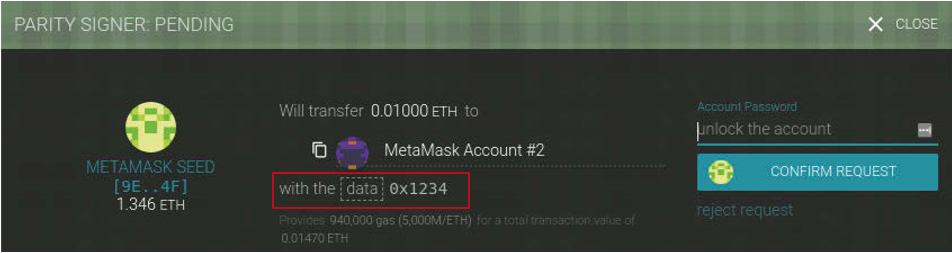
\includegraphics[width=\textwidth, keepaspectratio]{dataTransaction.png}
  \caption{Beispieltranskation an EOA mit gefülltem \textit{data}-Feld \cite[S.109]{antonopoulos_mastering_2019}}
\end{figure}
Relevant wird der Inhalt, wenn es sich bei der \textit{to} Adresse um einen Kontrakt handelt. Der Inhalt wird dann von der EVM als ein Funktionsaufruf interpretiert. Unsere Transaktion $T_x$ soll die Funktion\\
\begin{verbatim}
  function deposit(string _depositReason) public payable {
    balances[msg.sender] += msg.value;
    reasons[msg.sender].push(_depositReason);
  }
\end{verbatim}
unseres Kontrakts aufrufen. Diese Funktion fügt den kontraktinternen Konto dem im \textit{value}-Feld übergeben Wert hinzu. Dabei muss als Parameter der Einzahlungsgrund genannt werden. 

Damit diese Funktion aufgerufen werden kann, muss der Funktionsaufruf der Spezifikation des Contract Application Binary Interface (ABI) entsprechen. % https://solidity.readthedocs.io/en/v0.6.6/abi-spec.html %
Das heißt der endgültige Inhalt setzt sich im allgemeinen aus dem Funktionsselektor und den Funktionsargumenten zusammen. Der Funktionsselektor teilt dem Kontrakt mit welche Funktion er ausführen soll und entspricht den ersten vier Bytes des Keccak-256-Hash, welches das meist genutzte Hash-Verfahren in Ethereum ist, des Funktionsprototypen. Laut ABI Spezifikation setzt sich der Funktionsprototyp aus dem Namen der Funktion und in Klammern folgend die einzelnen Parametertypen. Der Rückgabetyp einer Funktion ist nicht Teil des Funktionsprototyps.
Daraus resultiert folgender Prototyp für unsere Funktion: \texttt{deposit(string)}.
Dessen vollständiger Keccak256-Hash entspricht:
\begingroup
\fontsize{8pt}{10pt}\selectfont
\begin{center}
  \texttt{a26e11860cdb80ecca46e4f433c3c9533f6d37cdf0f6eb16343556cfdbcf47ec}
\end{center}
\endgroup
Somit entspricht \texttt{0xa26e1186} dem ABI konformen Funktionsselektor.\\
Unser Funktionsaufruf soll 1000000000000000000 Wei (entspricht einem Ether) auf das Konto einzahlen. Als Parameter übergeben wir "`Einzahlung"'. Um einen String ABI konform zu kodieren müssen wir den Offset angeben, ab dem der Inhalt unseres Parameter startet, konkatiniert mit der Länge des Strings und beides nach links auf 32 Byte mit Paddingsbytes aufgefüllt. Danach folgt der String in UTF-8 kodiert, welcher nach rechts auf 32 Bytes aufgefüllt wurde. In unserem Fall müssen wir 32 Zeichen überspringen (\texttt{0x20}). Der String ist 10 (\texttt{0xa}) Zeichen lang. Somit lautet die Kodierung unserer Funktionsargumente wie folgt: 
\begingroup
\fontsize{8pt}{10pt}\selectfont
\begin{center}
  \texttt{0x0000000000000000000000000000000000000000000000000000000000000020 \textbackslash} \\
  \texttt{000000000000000000000000000000000000000000000000000000000000000a \textbackslash} \\
  \texttt{45696e7a61686c756e6700000000000000000000000000000000000000000000}
\end{center}
\endgroup
Unsere Nutzlast, welche wir im \textit{data}-Feld nun eintragen müssen, erhalten wir aus der Konkatenation beider Kodierungen:
\begingroup
\fontsize{8pt}{10pt}\selectfont
\begin{center}
  \texttt{0xa26e1186 \textbackslash} \\
  \texttt{0000000000000000000000000000000000000000000000000000000000000020 \textbackslash} \\
  \texttt{000000000000000000000000000000000000000000000000000000000000000a \textbackslash} \\
  \texttt{45696e7a61686c756e6700000000000000000000000000000000000000000000}
\end{center}
\endgroup

Damit unser Kontrakt auch die 1 Ehter erhält müssen wir diese im \textit{value}-Feld eintragen. Unsere Funktion besitzt das Schlüsselwort \texttt{payable}, dieses wird bei Kontrakten verwendet um anzuzeigen, dass diese Funktion Ether annehmen kann. Dabei muss die im \textit{data}-Feld aufgerufene Funktion nicht zwingend auch \texttt{payable} deklariert sein. Die EVM such in dem Fall alle Funktionen durch, bis sie eine so deklarierte Funktion findet. Wenn keine Funktion \texttt{payable} deklariert wurde, gibt es meistens eine sogenannte Fallback-Funktion, welche keinen Funktionsnamen besitzt und alleinig dazu dient Ether entgegen zu nehmen und diese dem Kontrakt gut zuschreiben. Ist auch diese nicht definiert, wirft die EVM eine Exception und die Transaktion wird abgebrochen.
Man kann jedoch über das \textit{data}-Feld keinen Ether an den Kontrakt übergeben. Dies ist ausschließlich über das \textit{value}-Feld möglich. Damit der Kontrakt dieses Ether annimmt, muss die Funktion genau wie unsere Funktion mit dem Schlüsselwort \texttt{payable} deklariert sein. Akzeptiert die aufgerufene Funkntion kein Ether, so wird die sogenannte Fallback-Funktion aufgerufen, die den übergenenen Etherbetrag auf das Konto des Kontrakts gut schreibt. Ist auch diese nicht definiert, wird eine Exception geworfen und die Transaktion abgebrochen.% Gas muss trotzdem gezahlt werden. % Solidity Dokumentation %

Die letzte mögliche Kombination ist, wenn sowohl das \textit{value}- und \textit{data}-Feld leer sind. Dies ist ebenfalls eine gültige Transkation würde. Diese erfüllt jedoch keinen besonderen Zweck außer der Verwendung des bezahlten Gas und somit nur einer Senkung des eigenen Kontostands.
\subsection{Signatur}

\subsubsection{ECDSA}
\label{ecdsa}

\subsubsection{Multisignaturen}

\section{Transaktionsabwicklung}
Wir haben nun alle notwendigen Konzepte und Inhalte einer Ethereumtranskation kennengelernt. Im weiteren wird vorgestellt, wie unsere Transkation $T_x$ im Netzt verteilt wird und diese in der Blockchain aufgenommen wird.
Damit unsere Transaktion versendet werden kann, werden unsere Transaktionsdaten mit dem privaten Schlüssel des sendenden Accounts signiert\footnote{Es wird angenommen, dass ein eigener Node betrieben wird. Werden Anwendungen wie MetaMask verwendet übernimmt diese die Signierung} und anschließend mit RLP kodiert\cite{antonopoulos_mastering_2019}.
\subsection{Propagation}
Bevor die Transaktion über das Ethereumnetzwerk verbreitet wird, überprüft der lokale Node (oder der Node, welcher MetaMask verwendet) ob die Transaktion wirklich von der eigenen Adresse stammt. Ist dies der Fall wird die Transkation über das P2P-Netwerk versendet. Ein Node ist mit mindestens 13 weiteren Nodes verbunden\cite[S.123]{antonopoulos_mastering_2019}. Jeder dieser erhält die Transkation und validiert dieser. Wenn dies erfolgreich ist sendet der jeweilige Node die Transaktion an seine Nachbarn weiter \cite[S.123]{antonopoulos_mastering_2019}. So wird erreicht, dass die Transkation sehr schnell bei jedem Node im Ethereumnetzwerk angekommen ist. Die Transaktion erreicht somit auch sogenannte Miner Nodes. Diese Nodes speichern unsere Transaktion in ihrem \textit{Mempool}. Abhängig von unserer Platzierung in dieser Liste, wird die Transaktion an einem Zeitpunkt in einen Block aufgenommen. Sobald der der Block geschürft wurde, das heißt der \textit{Proof of Work} gefunden wurde, findet eine Zustandsänderung des Zustandsautomat statt. Das heißt, die Funktion des Kontrakts wird von der EVM ausgeführt und das Ehter von dem Senderaccount abgebucht und dem Konto des Kontrakts gutgeschrieben. Schließlich kann man unsere Transaktion in der Blockchain wiederfinden: % Link zur Transaktion in Etherscan %
\subsection{Speicherung}
% receipt

\section{Ausblick}

% Literatur
\bibliographystyle{splncs04.bst}
\bibliography{paper.bib}

\end{document}

